\documentclass[border=10pt]{standalone}
\usepackage{tikz}
\usetikzlibrary{calc}

\tikzset{
    colorful steps/.style={
        path picture={
            \foreach \c [count=\i from 0] in {#1} {
                \fill[\c] 
                    let \p1=($(path picture bounding box.east)-(path picture bounding box.west)$) in
                    ([xshift={(1-1/pow(2,\i))*\x1}]path picture bounding box.south west)
                    rectangle 
                    (path picture bounding box.north east);
            }
        }
    }
}

\begin{document}
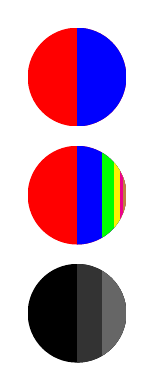
\begin{tikzpicture}

\node[colorful steps={red,blue}, circle, text width=1cm] at (0,0) {};

\node[colorful steps={red,blue,green,yellow,magenta,brown}, circle, text width=1cm] at (0,-1.5) {};

\node[colorful steps={black, black!80, black!60}, circle, text width=1cm] at (0,-3) {};

\end{tikzpicture}
\end{document}